\chapter{Materials and methods}\label{chap:MatlsMethds}
A series of batch shaking tests was conducted to test the sorption strength of waste-based biochars to PFAS, and to determine possible sorption mechanisms. Experiments to investigate how chain length affects sorption, both with and without the presence of soil, were conducted using six perfluorinated carboxylic acids (PFCAs) (C5-C10). Both single compound and a cocktail of C5-C10 batch tests were performed to determine attenuation factors. A methods flowchart is given in \cref{fig:methodoverview}. The main work and laboratory experiments were conducted in the environmental chemistry laboratory at the Norwegian Geotechnical Institute (NGI), Oslo, Norway. Quantification analysis of the batch test filtrates was performed by LC-MS/MS at the Institute for Chemistry, Norwegian University of Science and Technology (NTNU), Trondheim, Noway.

\begin{figure}[ht]
    \centering
    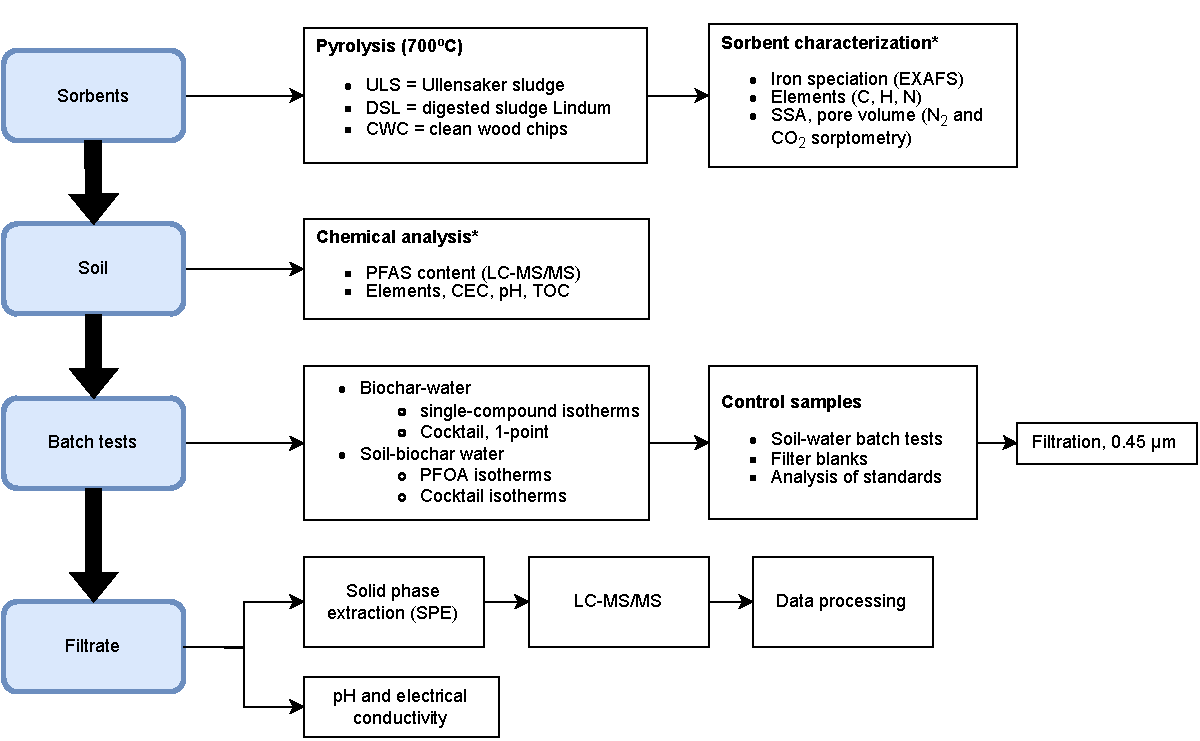
\includegraphics[width=0.94\textwidth]{Diagrams/Methods-General_overview_methods.pdf}
    \caption{Overview of the methods conducted for this thesis. * = analyses conducted by commercial laboratories or that were delegated to project partners.}
    \label{fig:methodoverview}
\end{figure}

\section{Biochar sorbents}
\subsection{Feedstock}
Three feedstocks were selected for use as sorbents for the sorption experiments:

\begin{itemize}
    \item \textbf{Ullensaker sludge (\acrshort{ULS})}: raw sewage sludge biosolids from Ullensaker wastewater treatment plant located North-East of Oslo, Norway. 
    \item \textbf{Digested sludge Lindum (\acrshort{DSL})}: a solid residue (digestate) left over from anaerobic digestion of food waste and organic material for the production of commercial biogas.
    \item \textbf{Clean wood chips (\acrshort{CWC})}: clean, fresh softwood timber, without additives, that has been shredded, dried, and compressed into 8 mm pellets. The wood pellets were commercially available from Hallingdal Trepellets (Kleivi næringspark, Ål, Norway)
\end{itemize}

These feedstocks were dried and pelletized before pyrolysis.

\subsection{Pyrolysis}
The ULS, DSL, and CWC biochars were provided as sample biochars for the sorption experiments conducted for this thesis. The biochars were produced at Lindum AS (Drammen, Norway) by using Biogreen\textsuperscript{\textcopyright} technology, provided by the French company, ETIA (Evaluation Technologique, Ingénierie et Applications). The CWC, ULS, and DSL biochars were produced by slow pyrolysis at 700 \textdegree C and a residence time of 20 minutes for CWC and 40 minutes for ULS. 

First, the pyrolysis chamber was electrically heated to a stable pyrolysis temperature. Feedstock pellets were added to a feeding container where a heated rotating screw (Spirajoule\textsuperscript{\textregistered}) led the feedstock through the pyrolysis chamber for the desired residence time. The biochar product was then transported to an external collection container where it was dispensed into sampling bags \cref{fig:pellets}. Syn-gas from pyrolysis was led through a condensing pipe, and condenses into bio-oil at two points, depending on boiling point. Syn-gas that does not condense at this point was led into a combustion chamber where a steady inflow of propane ensured clean combustion of the remaining compounds.

\begin{figure}
    \centering
    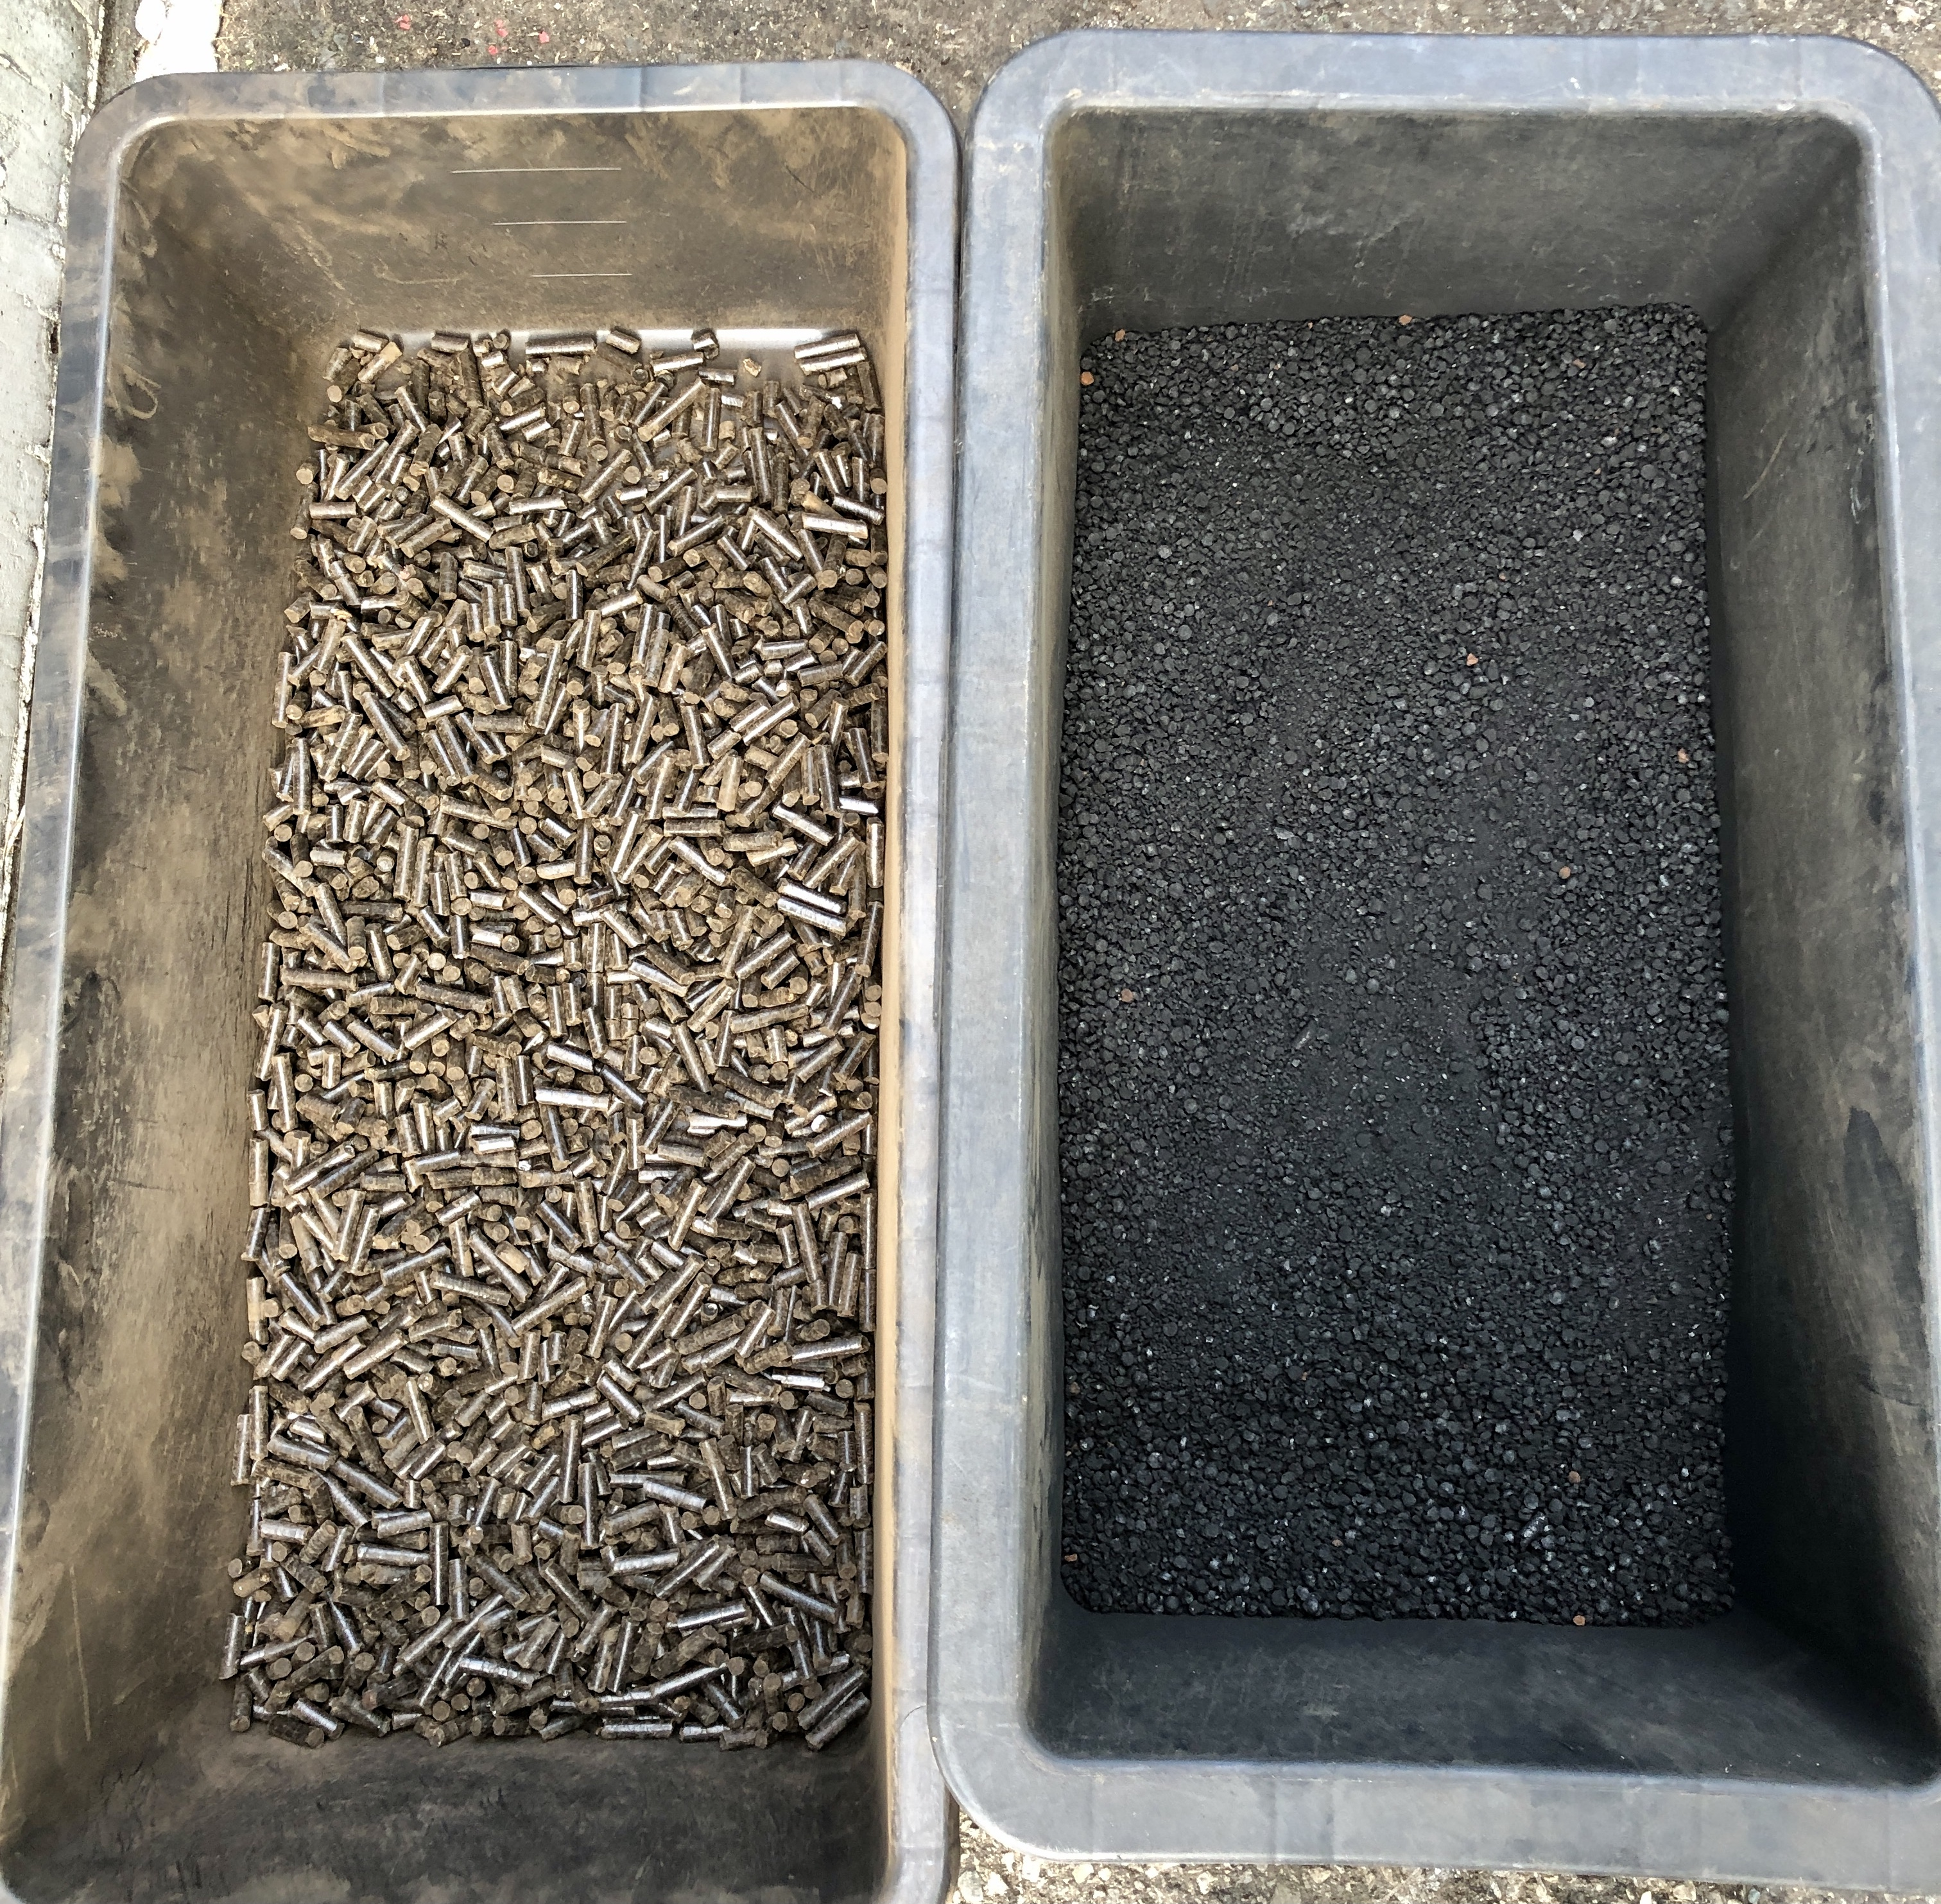
\includegraphics[width=0.5\linewidth,scale=0.6]{Bilder/Pyrolysis/Pellets.png}
    \caption{DSL feedstock pellets (left) and DSL biochar (right).}
    \label{fig:pellets}
\end{figure}

A biochar sub-sample (100 g) was taken by random grab-sampling from the bulk volume ($\sim$ 5 kg) of the biochar produced during pyrolysis. The biochars were crushed using a ball mill (Retsch ISO 9001) at 50 rpm for 5 minutes, then sieved into fine-powdered biochar (D \textless 1 mm), and transferred to LDPE zipper bags for storage (4 \textdegree C). 

\subsection{Biochar properties}
\subsubsection{Surface area and pore volume}
Total specific surface area (SA) and pore volume (PV) were determined by nitrogen ($\mathrm{N_2}$) and carbon dioxide ($\mathrm{CO_2}$) gas sorptiometry conducted by research partners at the Particle Engineering Research Center, University of Florida (Gainesville, USA) using a Quantachrome Autosorb 1 surface area analyzer according to the methods described by \cite{kwon2005}. $\mathrm{N_2}$ sorptiometry was performed at the boiling point for liquid nitrogen (-195.8 \textdegree C). Due to slow diffusion at this low temperature, $\mathrm{N_2}$ cannot enter the smallest pores $<$1.5 nm, and thus, sorption of $\mathrm{N_2}$ represents the largest pores of \textgreater 1.5 nm. $\mathrm{CO_2}$ sorptiometry was performed at 0 \textdegree C, enabling the gas to diffuse into smaller nanopores between 0.4-1.5 nm. $\mathrm{N_2}$ SA was interpreted using both Brunauer, Emmett and Teller (BET) and density functional theory (DFT). $\mathrm{N_2}$ PV was interpreted with Barret-Joyner-Halenda (BJH) and DFT. $\mathrm{CO_2}$ SA and PV were interpreted using DFT. 

\subsubsection{Element analysis}
The analysis of biochar total element composition was performed by project partners at the Norwegian University of Life Sciences (NMBU, Ås, Norway) according to DIN 51732. Total carbon (C) was analyzed by the dry combustion method described by \cite{nelson1983total}. The samples were crushed with a mortar before quantification by a Leco CHN628 from Leco Corporations (Sollentuna, Sweden). The sample was combusted at 1050 \textdegree C until complete oxidation of the C into $\mathrm{CO_2}$. The concentration of $\mathrm{CO_2}$ was measured by an infrared cell. Total nitrogen (N) was determined according to the \textit{Dumas} method \citep{Dumas1983total} by the same principles as that of total C. The N-containing constituents were reduced by copper into $N_2$. Nitrogen gas concentration was measured by thermal conductivity, also performed with Leco CHN628. 

The biochar composition of the remaining main elements (Ca, Fe, K, Mg, Na, P, S and Si) and trace elements (As, Ba, Cd, Co, Cr, Cu, Mo, Ni, Pb, Sr, V and Zn) were determined by $\mathrm{NO_3}$-digestion at 260 \textdegree C in an Ultraclave from Milstone, followed by dilution and analysis using either an Agilent Triple QQQ 8800 ICP-MS with a reaction-collision cell (As, Ba, Cd, Co, Cr, Cu, Mo, Ni, Pb, S, Sr and V), or an ICP-OES (Ca, Fe, K, Mg, Na, P, Si and Zn). In these analyses, the NJV 94-5 and NCS ZC 73007 certified reference materials were used for quality control purposes.

\subsubsection{Iron speciation}
Iron speciation of DSL and ULS were analyzed by Fe K-edge X-ray absorption fine structures (EXAFS) at the synchrotron SOLEIL (Gif-sur-Yvette, France) (beamline SAMBA) by one of the project partners at NGI, with practical assistance by the author of this thesis. To prepare the biochars for analysis, each sample ($\sim$50 mg) was crushed to a fine powder in a mortar (250$\mathrm{\mu m}$). The samples were then mixed with boron nitride (BN, 300 mg) to a homogeneous powder, and then pelletized. The BN matrix was used for sample dilution because it absorbs very little of the photon beam at the absorption edge. The resulting biochar pellets were analyzed by X-ray absorption spectroscopy.

The overall principle of EXAFS is to determine the structural composition of a sample by examining its X-ray absorption spectrum. This plots absorbance, $\mu x$, as a function of photon energy, $eV$ \citep{vlaica2004exafs}. The sample is then submitted to an X-ray beam where a spectrophotometer measures the beam's intensity as it passes through the sample. The difference in intensity, measured both before and after passing through the sample, is translated into an absorption coefficient, following Beer-Lambert's Law: 

\begin{equation}\label{eq:absorbance}
    \mu x = \log \frac{I}{I_0}
\end{equation}

where $\mu x$ is a dimensionless absorbance coefficient ($AU$), $I$ is the transmitted light intensity, and $I_0$ is the incident light intensity. The energy of the photon beam can be determined by the angle of a crystal monochromator, tuned so that the sample is bombarded by a range of photon energies between which the absorption edges of the target element is expected to be located \citep{vlaica2004exafs}. An adsorption K-edge occurs when the transmitted photon energy equals the energy required to excite a core electron, and is observed as a vertical jump (K) in $\mu x$ on the spectrum \citep{vlaica2004exafs}. The neighboring elements interfere with the photon wave which then translates into oscillations on the absorption spectrum following the absorption edge. Each element has a different oscillation pattern. The frequency and amplitude of these oscillations are (partially) determined by the type and number of neighboring atoms. The absorption edge energy and oscillations thus contain information on the valency of the element, as well as the number and type of neighboring atoms, that is to say, the element speciation.

Fe(II) species will have their K edge at a lower energy than Fe(III) species because a higher photon energy is required to excite an electron from the more electronegative Fe(III). In addition, the following oscillation pattern will differ depending on the Fe mineral. The different iron species present in the sample can be derived by interpreting the resulting X-ray absorption spectrum.

%%%%%%%%%%%%%%%%%%%%%%%%%%%%%%%%%%%%%%%%%%%%%%%%%%%%%%%%%%%%%%%%%%%%%%%%%%%%%%%%%%%%%%%%%%%%%%%%%%%%%%%%%%%%%%%

\section{PFAS analytes}\label{sec:PFCAanalytic}
6 perfluorinated carboxylic acids (PFCAs) were selected as target compounds for the batch test experiments. These were: \acrshort{PFPeA}, \acrshort{PFHxA}, \acrshort{PFHpA}, \acrshort{PFOA}, \acrshort{PFNA}, \acrshort{PFDA}, with perfluorinated carbon units 4-9 respectively (Full names are listed in \cref{tab:PFCAs}). 10 mL stock solutions for each PFCA were prepared by weighing the pure compound salt/liquid (\cref{tab:PFCAs}), and then dissolving them in methanol in volumetric flasks. Additional safety precautions were taken during this procedure by using double latex gloves. 

Two spiking standards at high (STD1) and low (STD2) concentrations were prepared from the stock solution used for spiking the batch tests at various concentrations (standard concentrations in \cref{apptab:standards}). The working standards were analyzed by LC-MS/MS of a twice diluted standard at an optimum concentration for the instrument calibration curve (10-20 $\mathrm{\mu g/L}$). All further calculations of spike dilutions were corrected by means of the measured standard concentrations. See \cref{appSec:IsothermSetup} for expected vs. analytical concentrations. A detailed description of the LC-MS/MS analytical procedure is given in \cref{sec:LCMS}. 

\begin{table}
\centering
\caption{PFAS compounds investigated in this study. PFCs correspond to the number of perfluorinated carbon units in the chain. Note: PFCAs appear in dissociated form at environmentally relevant pH's due to low $pK_a$'s.}
\adjustbox{max width=\textwidth}{
\label{tab:PFCAs}
\begin{tabular}{@{}lcccclc@{}}
\toprule
\multicolumn{1}{c}{Chemical} & Acronym & Short & CAS number & Molecular structure & Stock form & Purity \\ \midrule
& & & & & &\\
\smash{\raisebox{4ex}{Perfluoropentanoic acid}}  & \smash{\raisebox{4ex}{PFPeA}} & \smash{\raisebox{4ex}{C5}} & \smash{\raisebox{4ex}{2706-90-3}} & \chemfig[atom style={scale=0.4}]{O=[:90](-[:30,,,1]OH)-[:150](-[:112.5]F)(-[:67.5]F)-[:210](-[:292.5]F)(-[:247.5]F)-[:150](-[:112.5]F)(-[:67.5]F)-[:210](-[:270]F)(-[:150]F)-[:210]F} & \smash{\raisebox{4ex}{liquid}} & \smash{\raisebox{4ex}{\textgreater 97 \%}} \\
& & & & & &\\
\smash{\raisebox{4ex}{Perfluorohexanoic acid}} & \smash{\raisebox{4ex}{PFHxA}}  & \smash{\raisebox{4ex}{C6}} & \smash{\raisebox{4ex}{307-24-4}} & \chemfig[atom style={scale=0.4}]{O=[:90](-[:30,,,1]OH)-[:150](-[:112.5]F)(-[:67.5]F)-[:210](-[:292.5]F)(-[:247.5]F)-[:150](-[:112.5]F)(-[:67.5]F)-[:210](-[:292.5]F)(-[:247.5]F)-[:150](-[:210]F)(-[:150]F)-[:90]F} & \smash{\raisebox{4ex}{liquid}} & \smash{\raisebox{4ex}{\textgreater 97 \%}} \\
& & & & & &\\
\smash{\raisebox{4ex}{Perfluoroheptanoic acid}} & \smash{\raisebox{4ex}{PFHpA}} & \smash{\raisebox{4ex}{C7}} & \smash{\raisebox{4ex}{375-85-9}} & \chemfig[atom style={scale=0.4}]{O=[:90](-[:30,,,1]OH)-[:150](-[:67.5]F)(-[:112.5]F)-[:210](-[:247.5]F)(-[:292.5]F)-[:150](-[:67.5]F)(-[:112.5]F)-[:210](-[:247.5]F)(-[:292.5]F)-[:150](-[:67.5]F)(-[:112.5]F)-[:210](-[:150]F)(-[:210]F)-[:270]F} & \smash{\raisebox{4ex}{crystalline}} & \smash{\raisebox{4ex}{\textgreater 99 \%}} \\
& & & & & &\\
\smash{\raisebox{4ex}{Perfluorooctanoic acid}} & \smash{\raisebox{4ex}{PFOA}}  & \smash{\raisebox{4ex}{C8}} & \smash{\raisebox{4ex}{335-76-2}}  & \chemfig[atom style={scale=0.4}]{O=[:90](-[:30,,,1]OH)-[:150](-[:67.5]F)(-[:112.5]F)-[:210](-[:247.5]F)(-[:292.5]F)-[:150](-[:67.5]F)(-[:112.5]F)-[:210](-[:247.5]F)(-[:292.5]F)-[:150](-[:67.5]F)(-[:112.5]F)-[:210](-[:247.5]F)(-[:292.5]F)-[:150](-[:90]F)(-[:150]F)-[:210]F} & \smash{\raisebox{4ex}{powder}} & \smash{\raisebox{4ex}{\textgreater 95 \%}} \\
& & & & & &\\
\smash{\raisebox{4ex}{Perfluorononaoic acid}}  & \smash{\raisebox{4ex}{PFNA}} & \smash{\raisebox{4ex}{C9}} & \smash{\raisebox{4ex}{375-95-1}} & \chemfig[atom style={scale=0.4}]{O=[:90](-[:30,,,1]OH)-[:150](-[:112.5]F)(-[:67.5]F)-[:210](-[:292.5]F)(-[:247.5]F)-[:150](-[:112.5]F)(-[:67.5]F)-[:210](-[:292.5])(-[:247.5]F)-[:150](-[:112.5]F)(-[:67.5]F)-[:210](-[:292.5]F)(-[:247.5]F)-[:150](-[:112.5]F)(-[:67.5]F)-[:210](-[:270]F)(-[:210]F)-[:150]F} & \smash{\raisebox{4ex}{crystalline}} & \smash{\raisebox{4ex}{\textgreater 97 \%}} \\
& & & & & &\\
\smash{\raisebox{4ex}{Perfluorodecanoic acid}}  & \smash{\raisebox{4ex}{PFDA}}  & \smash{\raisebox{4ex}{C10}} & \smash{\raisebox{4ex}{335-67-1}} & \chemfig[atom style={scale=0.4}]{O=[:90](-[:30,,,1]OH)-[:150](-[:112.5]F)(-[:67.5]F)-[:210](-[:292.5]F)(-[:247.5]F)-[:150](-[:112.5]F)(-[:67.5]F)-[:210](-[:292.5]F)(-[:247.5]F)-[:150](-[:112.5]F)(-[:67.5]F)-[:210](-[:292.5]F)(-[:247.5]F)-[:150](-[:112.5]F)(-[:67.5]F)-[:210](-[:292.5]F)(-[:247.5]F)-[:150](-[:210]F)(-[:150]F)-[:90]F} & \smash{\raisebox{4ex}{flakes}} & \smash{\raisebox{4ex}{\textgreater 98\%}} \\
& & & & & &\\ \bottomrule
\end{tabular}}
\end{table}

\section{Batch tests \label{sec:batch}}
Batch testing is a laboratory method that involves shaking biochar in a closed container using a specified water-to-solid (L/S) ratio, contact time, and different concentrations of PFAS. After shaking, the concentration of PFAS in the water phase is analyzed. An illustration of the batch test experimental procedure used for PFAS and biochar in this thesis is shown in \cref{fig:batchtest_setup}.

\begin{figure}[htb]
    \centering
    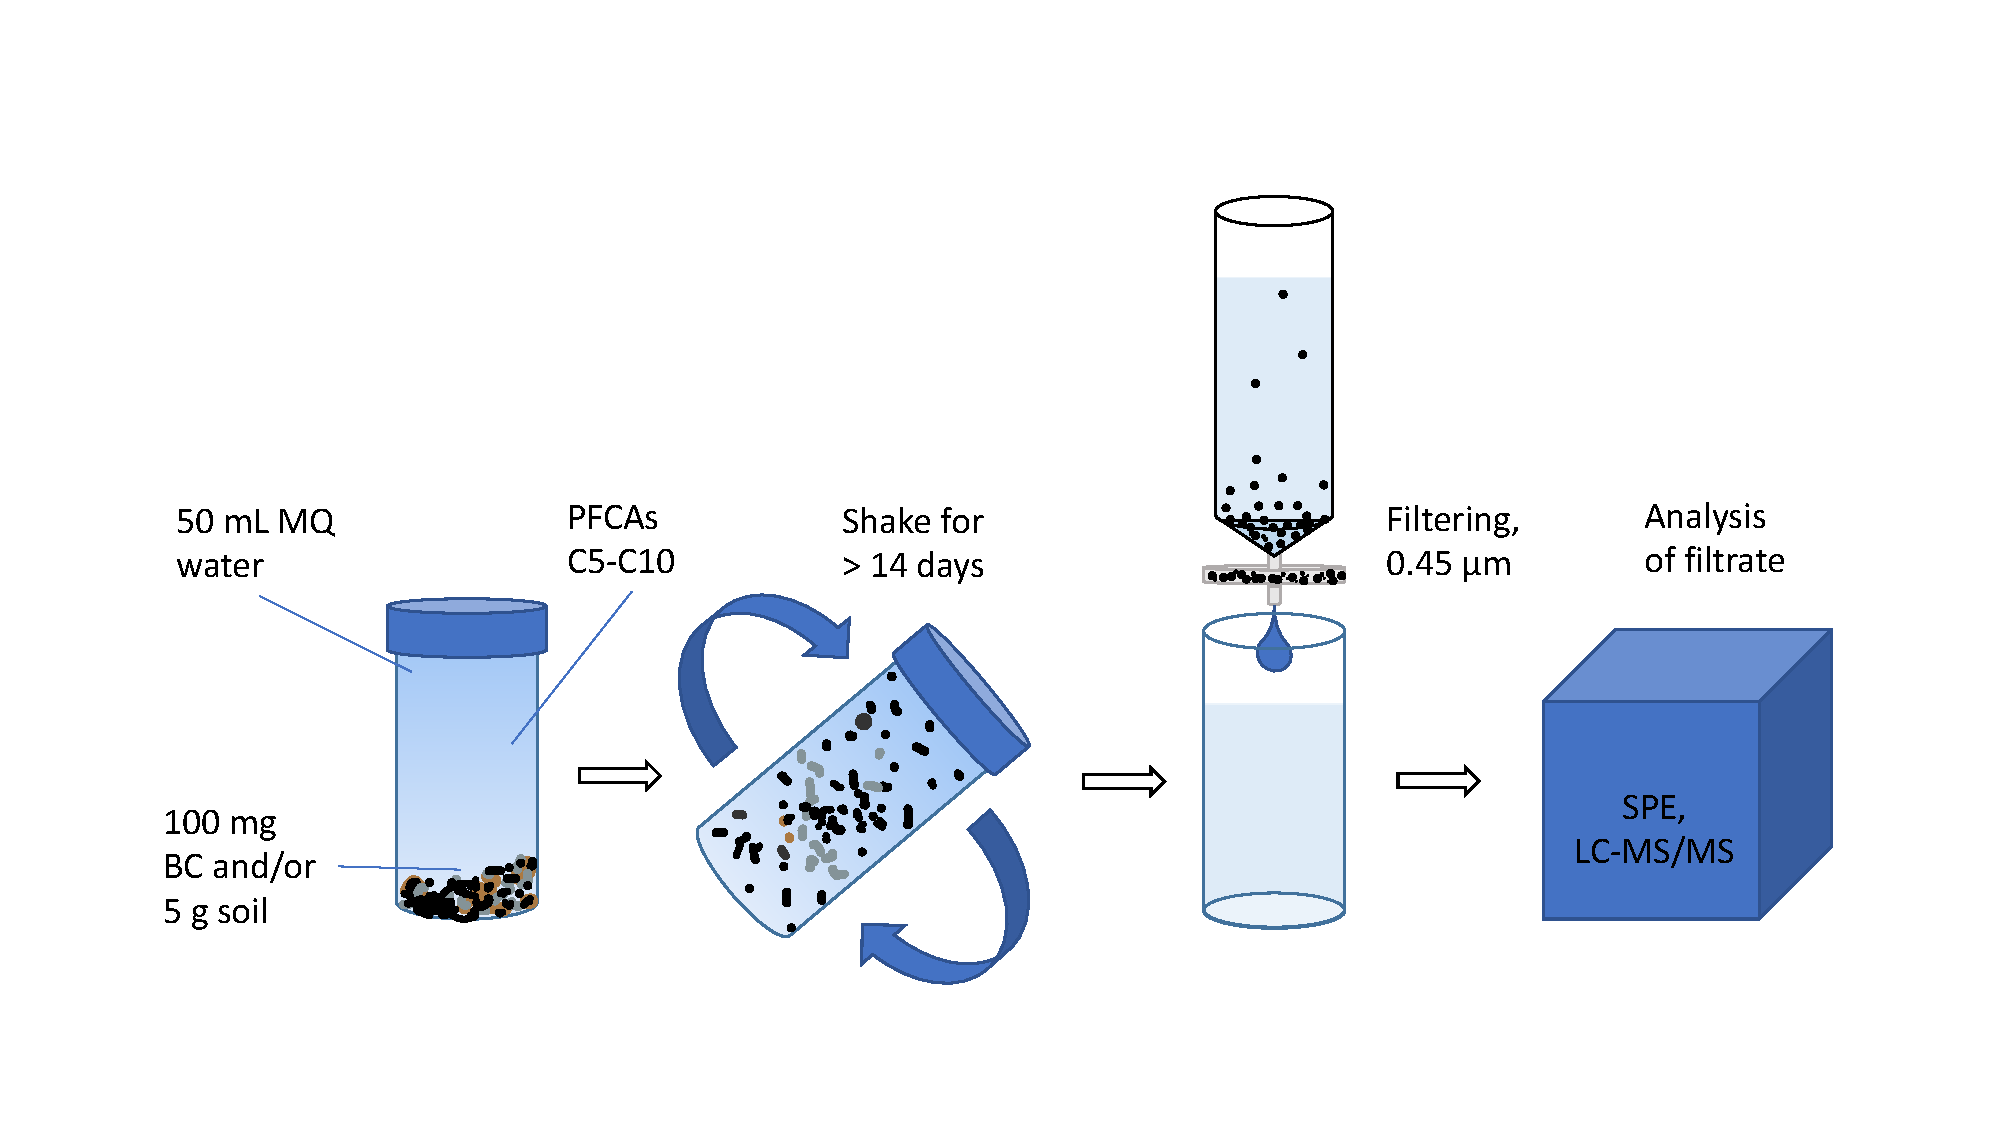
\includegraphics[width=\textwidth,trim={0 2cm 0 3.2cm},clip]{Diagrams/Batch_test.pdf}
    \caption{Experimental procedure for the laboratory batch shaking tests.}
    \label{fig:batchtest_setup}
\end{figure}

The batch tests prepared in this thesis were used to determine sorption isotherms for the biochars. A sorption isotherm is a curve that represents the distribution of a substance between the aqueous and sorbed phase at different concentrations \citep{limousin2007sorption}. Sorption of PFAS to biochar is weakened at higher concentrations caused by a gradual saturation of sorption sites \citep{schwarzenbach2005environmental}. This means that sorption isotherms for biochar are linear at low concentrations and gradually become non-linear at higher concentrations. When designing the batch test experiments for this thesis, the goal was to represent sorption of PFAS across both the linear and non-linear regions, this to determine at which concentration BC sorption sites.... what?  A more detailed description of this trend, called attenuation, is provided in \cref{sec:soilattenuation}. 

\subsection{PFAS spike concentrations}
To achieve detectable equilibrium aqueous concentrations ($C_w$), determining appropriate spike concentrations was based on several factors: 1) obtaining biochar-water distribution coefficients ($K_{BC}$) for the corresponding PFCAs from literature \cite{Xiao2017} \cref{apptab:Kbc}, 2) biochar dose, 3) LOQ of the analytical method (\cref{apptab:LOQ}), and 4) available volumes of pipette tips. The relationships between $K_{BC}~\mathrm{(L~kg^{-1})}$, the sorbed concentration, $C_s~\mathrm{(\mu g~kg^{-1})}$, and the freely dissolved aqueous concentration, $C_w~\mathrm{(\mu g~L^{-1})}$, are expressed as:

\begin{align}
    \label{eq:Kbc1}
    K_{BC} = \frac{C_s}{C_w}
\end{align}

and was used to estimate the expected $C_w$. By rearranging \cref{eq:Kbc1}, $C_w$ can be expressed as a function of the mass PFCA spiked ($m_{TA}$), the estimated $K_d$, the biochar dose ($m_{BC}$), and sample water volume ($V_w$):

\begin{align}
    \label{eq:Cw2}
    C_w=\frac{\frac{m_{PFAS}}{\left (\frac{m_{BC}\times K_{BC}}{V_w}\right)+1}}{V_w}
\end{align}

The lowest spike concentration for each isotherm was established as two times the method LOQ in order to account for uncertainties when estimating resulting $C_w$. The remaining points were spread evenly over a $10^4$ concentration interval. 

Two preliminary batch tests were prepared to check how well the estimates from points 1) - 4) above matched the expected sorption strength of the biochar samples. A description of the preliminary tests is given in \cref{appSec:IsothermSetup}).

\begin{figure}[tb]
    \centering
    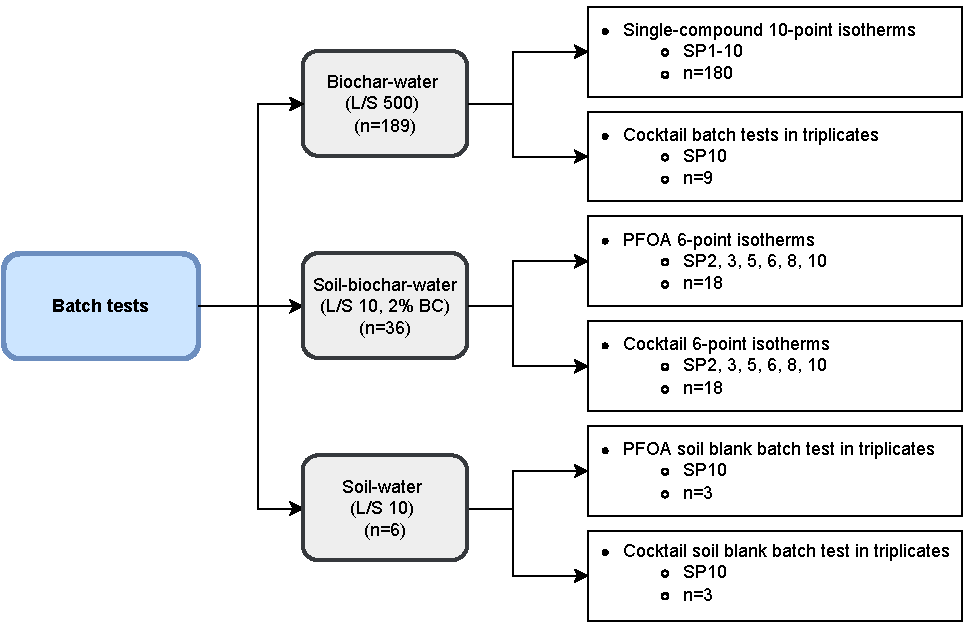
\includegraphics{Diagrams/Methods-Page-9.pdf}
    \caption{Experimental design of the batch tests prepared in this study. \acrshort{SC} = spike concentration (the acronym was changed to SP in the remaining discussions). SP10 = highest spiked concentration.}
    \label{fig:batchtests_flowchart}
\end{figure}

\subsection{Preparation of batch test \label{sec:batchtests}}
An overview of the experimental design of the batch tests is given in \cref{fig:batchtests_flowchart}. The batch tests were prepared with a liquid-to-solid mass ratio (L/S) of 500 for biochar, and an L/S of 10 for soil amended with 2\% biochar in accordance with CEN EN 12457, and with modifications described in \citep{Hale2017fire, kupryianchyk2016biochar}. The different batch test categories prepared were:

\begin{itemize}
    \item \textbf{BC-single}: biochar-water spiked with single PFCAs
    \item \textbf{BC-mix}: biochar-water spiked with a PFCA cocktail
    \item \textbf{BC-soil-PFOA}: soil-biochar-water spiked with single PFOA only
    \item \textbf{BC-soil-mix}: soil-biochar-water spiked with a PFCA cocktail
    \item \textbf{Soil-single}: soil-water spiked with single PFCAs
    \item \textbf{Soil-mix}: soil-water spiked with a PFCA cocktail
\end{itemize}

All samples were prepared in 50 mL polypropylene (PP) centrifuge tubes that were rinsed three times with 50\% MeOH to extract any potential PFAS contamination prior to sample preparation. 100$\pm$4 mg biochar and/or 5.000$\pm$0.005 g soil were added to the sample tubes and spiked with single PFCA compounds and a PFCA cocktail at the concentrations specified in \cref{tab:spikeConcentrations}. These were then filled with Milli-Q water to a final volume of 50 mL. A volume calibration was performed to control for variations in sample volumes and is in \cref{appSec:misclab}. Cocktail samples were spiked with the same relative amounts of each PFCA as the single-spike samples at SC10 (SC10-MIX and SC10-MIX-S). The concentrations spiked were compared to literature values for the critical micelle concentrations (CMC) of the different PFCAs, and were not an issue for the concentration range considered \citep{bhhatarai2011,ding2013physicochemical}. The samples were assured to contain $<$1\% MeOH, which is the upper limit to ensure that methanol does not influence sorption \citep{arvaniti2014}.

In order to reach equilibrium, batch tests were shaken end-over-end (9 rpm) and/or agitated on a shaking table (160 rpm) at room temperature (23\textdegree C) for at least 14 days \citep{kupryianchyk2016biochar}. The samples were filtered through a 0.45$\mathrm{\mu m}$ Minisart\textsuperscript{\textregistered} regenerated cellulose syringe filter into new \acrshort{PP} tubes using methods described in \cite{Sorengard2019}. Prior to filtration, the samples containing soil were centrifuged to remove as many particles from suspension as possible. However, filtration still required frequent filter changes due to clogging (up to three times per sample). Loss of biochar that adhered to the walls of the syringe was quantified in the event that a full mass balance was required for analysis of PFCA distribution \cref{appSec:misclab}. However, a 100\% mass balance was assumed when calculating the distribution between sorbent and water. The calculation was done by subtracting the initial spike concentration from the measured filtrate concentration.

\begin{table}
    \caption{Spike concentrations (SC) in $\mathrm{\mu g/L}$ used for the batch tests, corrected for the analytical standards.}
    \label{tab:spikeConcentrations}
    \adjustbox{max width=\textwidth}{%
    \begin{threeparttable}
    \begin{tabular}{lrrrrrrrrrrrr}
    \toprule
    Compound & SC1 & SC2 & SC3 & SC4 & SC5 & SC6 & SC7 & SC8 & SC9 & SC10 & SC10-MIX$^*$ & SC10-MIX-S$^\dagger$ \\ \midrule
    PFPeA & 0.019 & 21 & 43 & 64 & 86 & 107 & 128 & 150 & 171 & 191 & 191 & 283\\
    PFHxA & 0.033 & 37 & 73 & 110 & 146 & 184 & 220 & 256 & 292 & 330 & 330 & 836 \\
    PFHpA & 0.012 & 11 & 25 & 38 & 52 & 65 & 79 & 92 & 106 & 117 & 117 & 153\\
    PFOA & 0.195 & 216 & 435 & 651 & 871 & 1 087 & 1 302 & 1 522 & 1 742 & 1 953 & 1 953 & 1 974\\
    PFNA & 0.141 & 156 & 313 & 471 & 625 & 784 & 942 & 1 097 & 1 255 & 1 409 & 1 409 & 2 310\\
    PFDA & 0.383 & 425 & 850 & 1 275 & 1 700 & 2 126 & 2 551 & 2 976 & 3 401 & 3 830 & 3 830 & 5 288\\ \bottomrule
    \end{tabular}
\begin{tablenotes}
\item $^*$ cocktail of C5-C10 spiked to biochar-water batch tests
\item $\dagger$ cocktail of C5-C10 spiked to biochar-soil-water and soil-water batch tests
\end{tablenotes}
\end{threeparttable}}
\end{table} 

\subsection{Soil}
Soil used for batch tests in the presence of soil, was an unaged, sandy soil that was obtained from a remote field area, 17 km from Uppsala, Sweden (59.733 N, 17.667 E). The soil carbon content was determined through dry combustion according to ISO10694 (1995) using an elemental analyzer for macro samples (TruMac\textregistered CN, Leco corp, St. Joseph, MI, USA). This analysis was performed by research partners at the Swedish University of Agricultural Sciences (SLU), Uppsala, Sweden. The soil was classified as a fine sand (0.1 to 0.3 mm), with 1.3 \% TOC (pH 5.38 $\pm$ 0.02, CEC 2.63 $\pm$ 0.06 meqv 100 g\textsuperscript{-1}). Total element concentrations and exchangeable ion concentrations are presented in \cref{appSec:elements}, \cref{apptab:soil}. The soil was dried at 100 \textdegree C for 24 h, and then crushed and sieved to \textless 2 mm. 

\subsubsection{Filter clogging by soil}\label{sec:Soil}
Prior to filtration, the batch tests with soil contained different degrees of suspended particles despite being centrifuged. This made it difficult to filter the samples that contained the most suspended particles. Filtration led to clogged filters that had to be changed up to three times per sample. Frequently clogged filters likely resulted in reduced filter pore size associated with the fact that some DOC was retained. This may have led to underestimating $C_w$, and thereby overestimating $K_d$ for the soil samples. This, in turn, became an issue when deriving Freundlich distribution coefficients for biochar in the presence of soil. In the next section, additional considerations for calculating PFAS-distribution in batch tests with biochar in the presence of soil will be discussed. Filter blanks (\cref{sec:blanks}) were only prepared for BC-water samples that showed no significant effect (see \cref{apptab:FB}). Hence, the effect of reduced filter size by clogging could not be quantified. 

The resulting soil batch test filtrates varied in color \cref{fig:DOC}. The sludge biochar soil samples were more transparent than soil only, and soil-CWC. The remarkable difference in DOC could be attributed to DOC complexation with inorganic species present in the sludge chars, but not in CWC biochar, as inorganic ions are not a dominating component of clean wood-derived biochar. In summary, the observations made during filtration of the BC soil batch tests indicate that sewage sludge biochar binds DOC, and that DOC in the filtrate is potentially responsible for an underestimation of $C_w$, and hence, an overestimation of the soil-water distribution coefficient ($K_{d,s}$). 

\begin{figure}
    \centering
    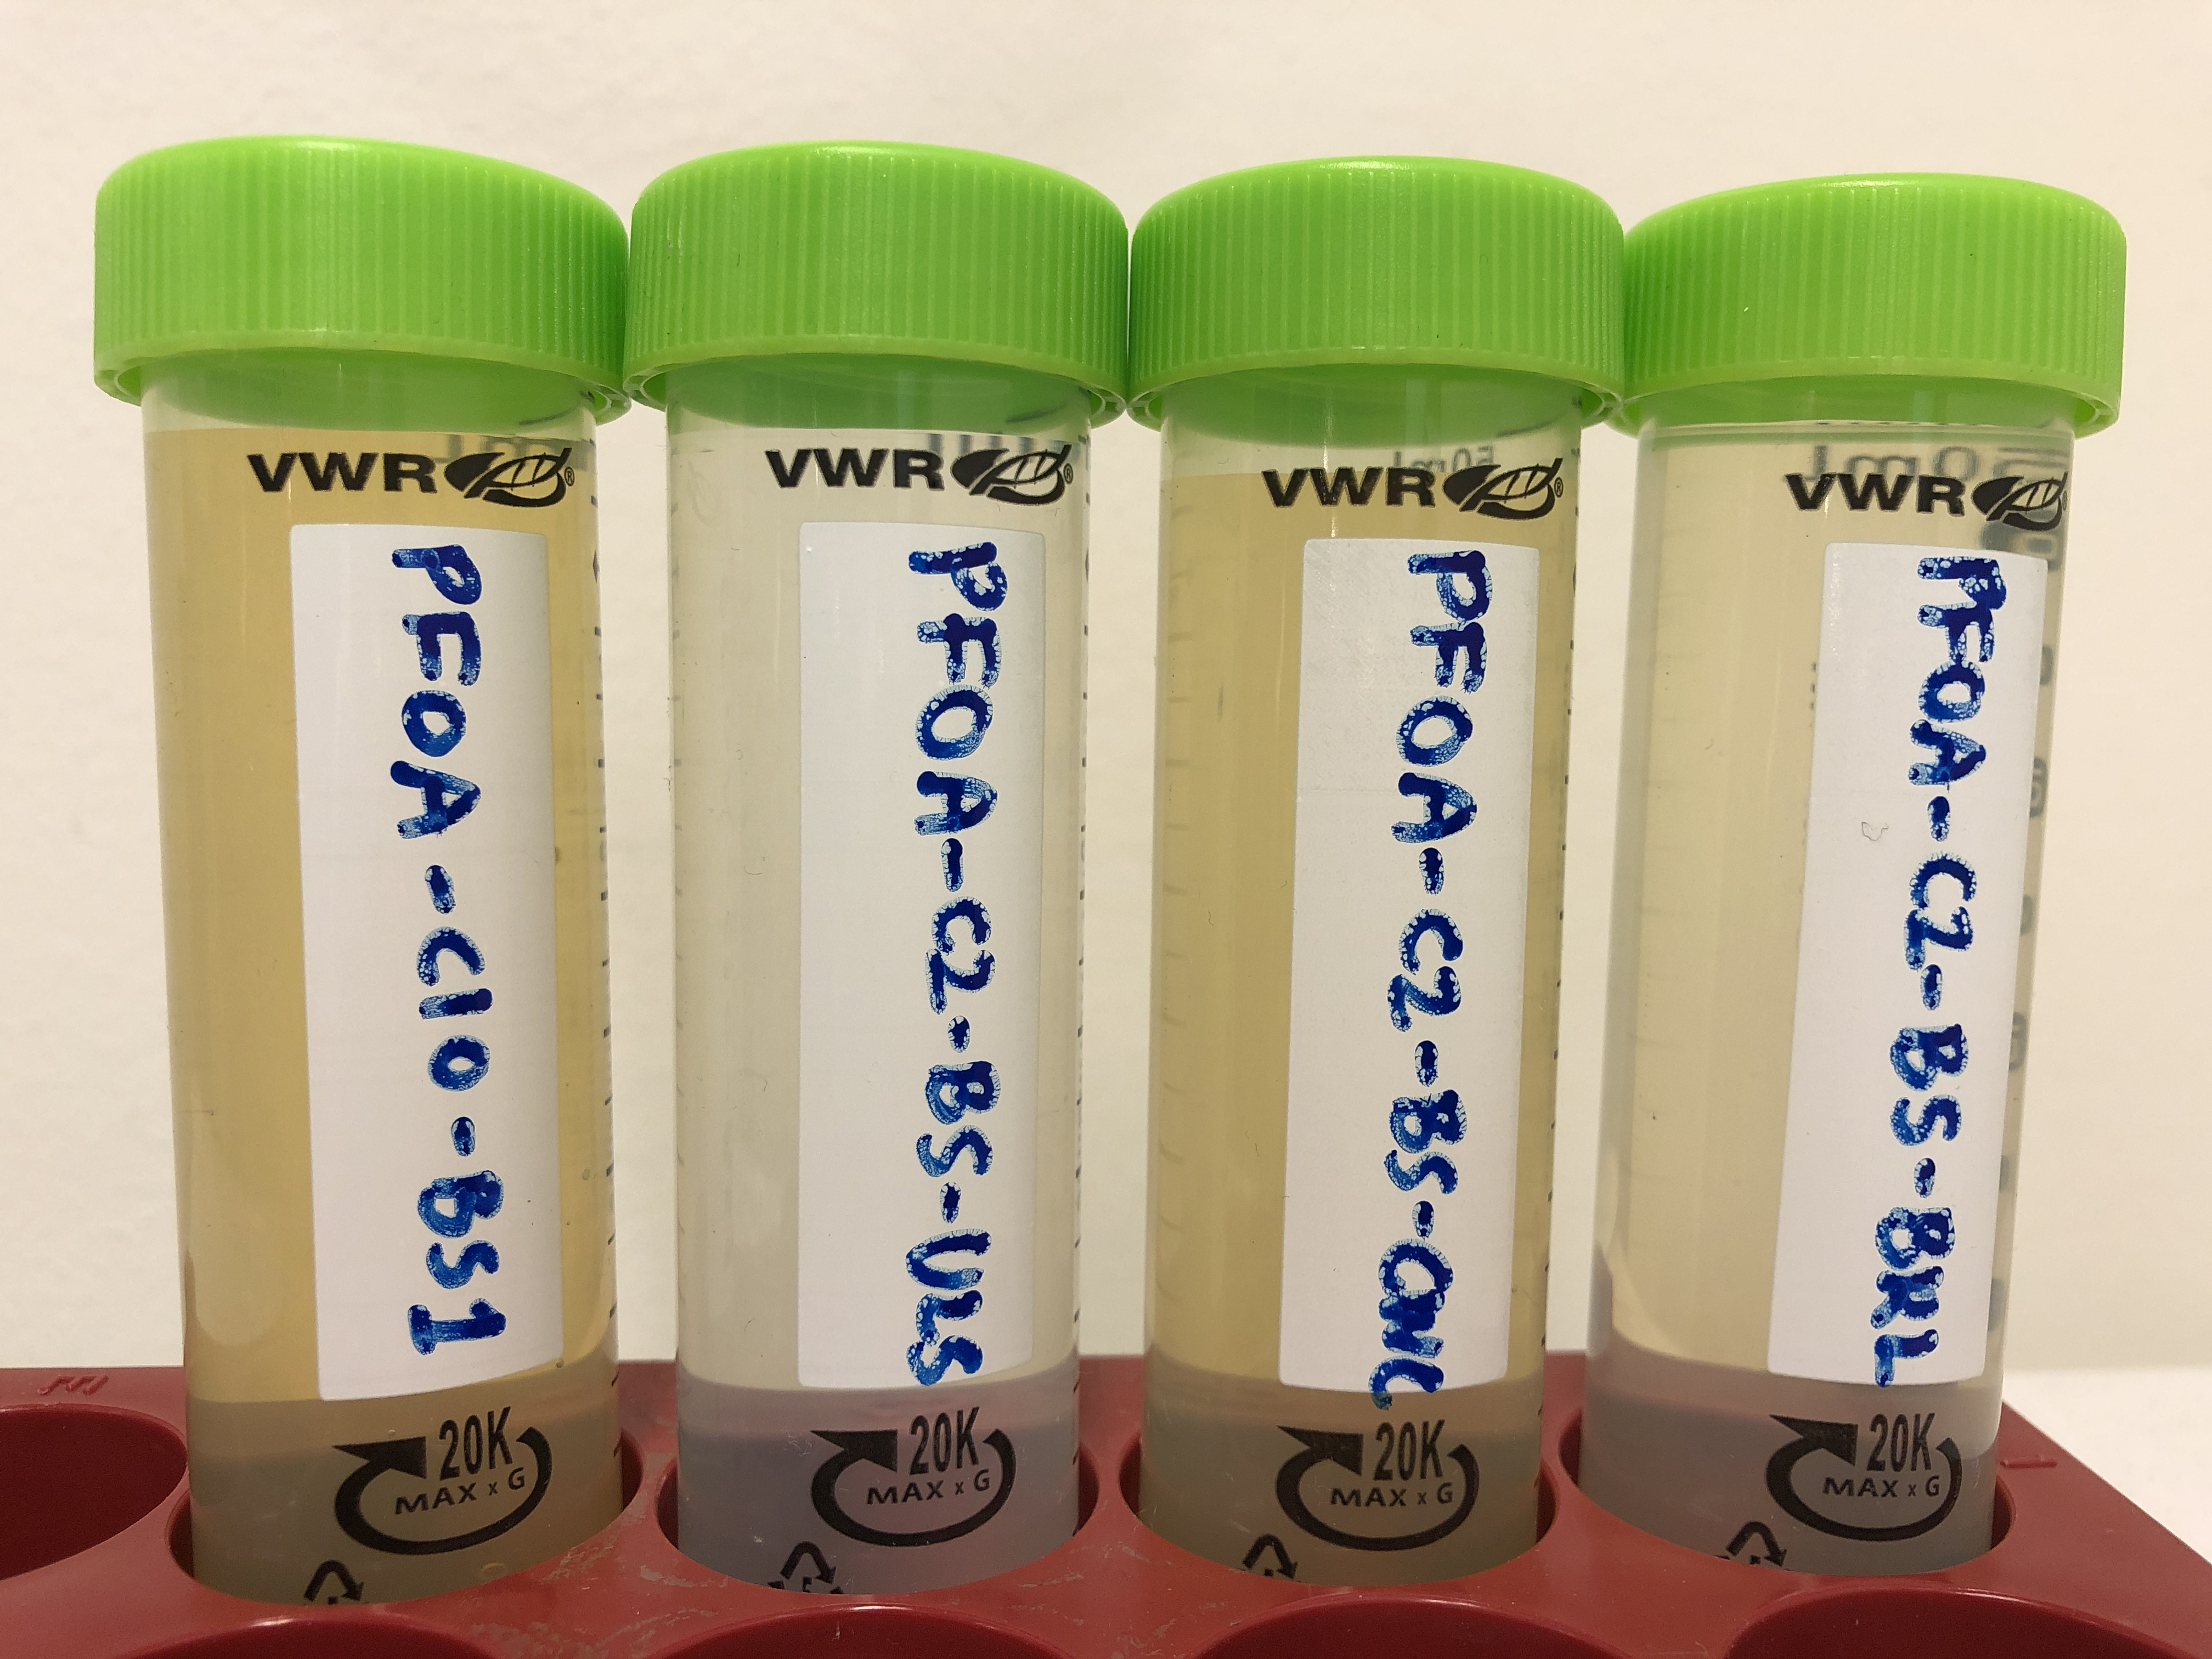
\includegraphics[width=0.7\textwidth]{Bilder/Samples/Filtrate_DOC.JPG}
    \caption{Color of filtrate for each biochar batch test. From left to right: soil only, soil+ULS, soil+CWC, and soil+DSL.}
    \label{fig:DOC}
\end{figure}

\subsection{Sample blanks \label{sec:blanks}}
To correct for potential PFCA-loss to the filter paper, and thereby underestimation of $C_w$, filtration blanks for each compound were prepared in triplicates for each PFCA at an optimum concentration range for the instrument (see \cref{sec:PFCAanalytic}).

\subsection{pH and electrical conductivity}
pH and conductivity were measured in a slurry of biochar and water (1:5). This involved pre-stirring (15 min) and then letting the particles settle (\textgreater 24 hrs) before measurement (n=3).

\section{Sorption models}
There are several empirical and theoretical models that can be used to fit a line between the concentration points that were generated from analysis of the batch test filtrates \citep{wang2020adsorption}. This study applied a linear sorption model to evaluate sorption to soil, and the Freundlich sorption model for the data points from batch tests that contained biochar. In this study, sorption isotherms were determined at equilibrium which was assumed to be reached after 14 days.

\subsection{The biochar-water distribution coefficient ($K_d$)}
Linear sorption assumes that sorption increases proportionally with concentration and is commonly used to determine distribution at one concentration point. Linear sorption is expressed by: 

\begin{equation}\label{eq:linear}
C_s = K_d \times C_w
\end{equation}

where $C_s$ is the sorbed amount, $C_w$ is the equilibrium aqueous concentration, and $K_d$ is the resulting distribution coefficient. Since sorption to biochar is non-linear, $K_d$-values cannot be extrapolated beyond the concentration point where they were determined at. Also, a comparison of $K_ds$ across samples can only be done if the $K_ds$ have the same equilibrium aqueous concentration.

\subsection{The Freundlich sorption model \label{sec:soilattenuation}}
The Freundlich sorption model provides a way of deriving distribution coefficients that represent solid-water phase distribution across a wider concentration range \citep{zhang2013sorption}. The Freundlich equation is expressed as:

\begin{equation} \label{eq:Freundlich}
    C_s = K_F \times C_{w}^{n_F}
\end{equation}

where $C_s$ is the amount sorbed in $\mathrm{\mu g/kg}$, $K_F$ is the Freundlich distribution coefficient in L/kg, $C_{w}$ is the equilibrium aqueous concentration in $\mathrm{\mu g/L}$, and $n_F$ is the coefficient of non-linearity. Because this model does not consider all sites on the adsorbent surface to be equal, but rather predicts that adsorption becomes progressively more difficult as more and more adsorbate accumulates, it is usually used for sorbents such as biochar that have heterogeneous surfaces\citep{yin2022insights,schwarzenbach2005environmental}. 
The Freundlich model assumes a log-normal sorption distribution \citep{schwarzenbach2005environmental}. Taking the $\log$ of each side of \cref{eq:Freundlich} results in a linear expression:

\begin{equation} \label{eq:FreundlichLinear}
    \log C_s = \log K_F + n_F \times \log C_{w}
\end{equation}

A linear regression line can be fitted between the $\log~C_w$ (x-axis) and $\log~C_s$ (y-axis) concentration points for each sample. The resulting regression equation is the Freundlich equation (\cref{eq:FreundlichLinear}) where the y-intercept is the Freundlich distribution coefficient ($\log~K_F$), and the slope is the coefficient of non-linearity ($n_F$). $n_F$ represents how linear the isotherm is within the concentration intervals achieved and is $<$1. $n_F$ is usually between 0.7 and 1.0 \citep{Cornelissen2005}.

The modeling of the soil-inclusive experiments is complicated since distribution behavior between soil-water and biochar-water must be considered together. The $K_d$ of soil must be determined separately and corrected in order to determine $K_F,BC$ in the presence of soil. Sorption to soil-only is most often linear and is therefore represented by \cref{eq:linear}. The mass balance for the distribution between water, soil and biochar (BC) is obtained by expanding the Freundlich equation (\cref{eq:Freundlich}). The mass balance between the three phases can be deduced as follows:

\begin{equation} \label{eq:massBalance1}
    m_{tot} = m_{w} + m_{s} + m_{BC}
\end{equation}

\begin{equation} \label{eq:massBalance2}
     m_{tot} = C_{w}V_{w} + C_sM_s + C_{bc}M_{BC}
\end{equation}

\begin{equation} \label{eq:massBalance3}
     m_{tot} = C_{w}V_{w} + K_dC_{w}M_s + K_{F}C_{w}^{n_F}M_{BC}
\end{equation}
 
where $m$ is the mass PFAS in ng or $\mathrm{\mu g}$, and $M$ is the mass soil or sorbent in kg. Substituting \cref{eq:massBalance3} in the Freundlich equation yields:

\begin{equation} \label{eq:FreundFit}
    m_{tot} - C_{w}V_{w} - K_dC_{w}M_s = K_{F}C_{w}^{n_F}M_{BC}
\end{equation}

\Cref{eq:FreundFit} contains the expression for the amount of PFAS in the BC on the left hand side, and an expression for the aqueous PFAS concentration on the right hand side. To get the linear Freundlich expression, the $\log$ of each side is taken:

\begin{equation} \label{eq:FreundLinSoil1}
   \log (m_{tot} - C_{w}V_{w} - K_dC_{w}M_s) = \log (K_{F}C_{w}^{n_F}M_{BC})
\end{equation}

Further modifications are made so as to simplify the Freundlich linear expression to $y = b + a \times x$:

\begin{equation} \label{eq:FreundLinSoil2}
    \log (m_{tot} - C_{w}V_{w} - K_dC_{w}M_s) = \log K_{F} + \log C_{w}^{n_F} + \log M_{BC}
\end{equation}

\begin{equation} \label{eq:FreundLinSoil3}
    \log (m_{tot} - C_{w}V_{w} - K_dC_{w}M_s) = \log K_{F} + n_F \times \log C_{w} + \log M_{BC}
\end{equation}

\begin{equation} \label{eq:FreundLinSoil4}
    \log (m_{tot} - C_{aq}V_{w} - K_dC_{w}M_s) - \log M_{BC} = \log K_{F} + n_F \times \log C_{w}  
\end{equation}

For each point on the isotherm, \cref{eq:FreundLinSoil4} can be plotted using $\log C_{w}$ on the $x$-axis, and $\log (m_{tot} - C_{aq}V_{aq} - K_dC_{aq}M_s) - \log M_{bc}$ on the $y$-axis. The resulting linear regression coefficients represent the same variables as the non-extended Freundlich expression (\cref{eq:FreundlichLinear}, that is, $n_F$ is the slope, and $log~K_F$ is the intercept. 

%%%%%%%%%%%%%%%%%%%%%%%%%%%%%%%%%%%%%%%%%%%%%%%%%%%%%%%%%%%%%%%%%%%%%%%%%%%%%%%%%%%%%%%%%%%%%%%%%%%%%%%%%%%%%%%%%%%%%%%%%%%%

\section{Instrumental analysis} \label{methods:instrAnalysis}

\begin{figure}
    \centering
    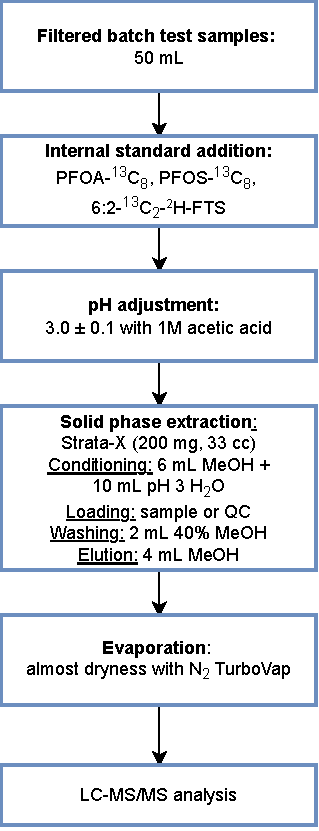
\includegraphics{Diagrams/Methods-Analytical_method.pdf}
    \caption{Schematic diagram of the analytical method applied for the determination of TCs in the batch test filtrates adapted from \cite{arvaniti2012diagram}.}
    \label{fig:analyticalMethod}
\end{figure}

\subsection{Solid-phase extraction (SPE)}
Solid-phase extraction (\acrshort{SPE}) is a sample-preparation method used to extract and concentrate a large-volume sample to produce a solvent extract. The extract can then be subjected to analyte quantification using LC-MS/MS. The sample is passed through a cartridge with a porous sorbent polymer which serves as the extraction agent, and strongly retains polar compounds. The sorbed analytes are then eluted with an appropriate solvent, evaporated, and finally reconstituted to the desired extract volume. All samples are spiked with a mix of internal standards (\acrshort{IS}s) to compensate for variations in extraction percentages and instrumental response by the mass spectrometer detectors \citep{arvaniti2014}.

Strata-X\textsuperscript{\textregistered} 200 mg/6mL cartridges, supplied by Phenomenex, were used for extracting the target compounds in the filtered water samples. The sorbent polymer was a surface modified styrene divinylbenzene (\cref{fig:StatPhase}) with a 33 $\mathrm{\mu m}$ average particle diameter, and a surface area of 800 m\textsuperscript{2} g\textsuperscript{-1}. The internal standards used were \textsuperscript{13}C\textsubscript{8}-perfluorooctanoic acid (\textsuperscript{13}C\textsubscript{8}-PFOA), \textsuperscript{13}C\textsubscript{8}-potassium perfluorooctanesulfonate (\textsuperscript{13}C\textsubscript{8}-PFOS-K), and 6:2-\textsuperscript{13}C\textsubscript{2}-\textsuperscript{1}H,\textsuperscript{2}H-perfluorooctane sulfonate (6:2 \textsuperscript{13}C\textsubscript{2}-FTS) where a working standard of the three isotopic PFASs was prepared in methanol at 1 ppm, from a 50 ppm analytical standard supplied by Sigma Aldrich.

A schematic description of the SPE protocol is provided in \cref{fig:analyticalMethod}. The filtered batch test samples were adjusted to pH $\sim$3 with 800 $\mathrm{\mu L}$ 1 M acetic acid. However, samples containing soil required adding at least double this amount to reach the same pH. pH strips were used to test the pH of five randomly selected samples from each batch of 20. All samples were then spiked with IS. SC1 and SC2 samples were spiked with 10 $\mathrm{\mu L}$ IS, and SC3-SC10 samples were spiked with 20 $\mathrm{\mu L}$ IS. The difference in the amount of IS for the two low-spike samples was due to the fact that a more concentrated extract was needed (0.5 mL vs. 1 mL) for these samples so as to avoid signals below instrumental \acrshort{LOQ}. The samples were vortexed prior to SPE.

The SPE cartridges were conditioned with 6 mL \acrshort{MeOH} and 10 mL pH 3 milli-Q water (acidified by 100\% acetic acid). MeOH was used for wetting to allow the mobile phase to flow into all the pores of the sorbent polymer. This ensured maximum chromatographic retention. Water with a low pH was used to protonate lone pair electrons on the polymer surface in order to maximize hydrophobic interaction with the analytes. The samples were loaded using glass pipettes, and allowed to pass through the cartridges by gravity. The flow rate was adjusted by modifying the opening of the cartridge openings by the use of LC liners so that the sample exited the cartridge as individual droplets.

After extracting the samples, the SPE cartridges were washed with 2 mL MeOH:\acrshort{MQ} (40:60, \% v/v) in order to remove any matrix interferences. The cartridges were then dried with a vacuum pump at 20 mmHg until the extraction agent was visible as a dry powder. The analytes were then eluted with 4 mL MeOH into 15 mL PP centrifuge tubes, and concentrated to $\le$0.5 mL using TurboVap\textsuperscript{\textregistered} at 40 \textdegree C, and nitrogen gas (N\textsubscript{2}) at 5 psi. The samples were reconstituted to 1 mL (0.5 mL for SCs 1 and 2) with MeOH and MQ, ending up at a final solvent ratio of 50:50 \% v/v. The extracts were transferred to LC vials using glass pipettes and stored at -19 \textdegree C until sample analysis took place. To minimize risk of contamination during laboratory work, working benches were cleaned with acetone and covered with aluminum foil. Sterilized PP tubes were used during all steps of the procedure.

\begin{figure}
    \centering
    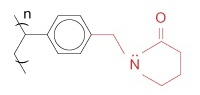
\includegraphics{Bilder/SPE_LCMS/mg_spe_strata-x.jpg}
    \caption{Polymer used as extraction agent in SPE, surface-modified styrene divinylbenzene.}
    \label{fig:StatPhase}
\end{figure}

\subsection{LC-MS/MS \label{sec:LCMS}}
Liquid chromatography separates compounds in a mixture based on polarity by using a stationary phase that retards hydrophobic compounds while allowing more polar compounds to pass through more quickly along with a polar mobile phase. Using high voltage, the compounds were then ionized into fragment ions which were detected by a mass spectrometer that determined the mass of the transitions. 

\begin{table}[tbh]
\centering
\caption{Ion transitions for the target analytes and internal standards in this study.}
\adjustbox{max width=\textwidth}{%
\begin{threeparttable}
\label{tab:transitions}
\begin{tabular}{ccccccl} \toprule
Compound &  Structure & Formula & M & Parent & Cone (V) & Transitions (CE)  \\ \midrule
& & & & & & \\
\multirow{2}{*}{PFPeA} &  \multirow{2}{*}{\chemfig[atom style={scale=0.5}]{O=[:90](-[:30,,,1]OH)-[:150](-[:112.5]F)(-[:67.5]F)-[:210](-[:292.5]F)(-[:247.5]F)-[:150](-[:112.5]F)(-[:67.5]F)-[:210](-[:270]F)(-[:150]F)-[:210]F}} & \multirow{2}{*}{$\mathrm{C_5HF_9O_2}$} & \multirow{2}{*}{264.05} & \multirow{2}{*}{262.97} & \multirow{2}{*}{20} & \multirow{2}{*}{262.97 $\rightarrow$ 219 (8)} \\
& & & & & & \\
& & & & & & \\
 &  &  &  &  &  &    \\
\multirow{2}{*}{PFHxA} &  \multirow{2}{*}{\chemfig[atom style={scale=0.5}]{O=[:90](-[:30,,,1]OH)-[:150](-[:112.5]F)(-[:67.5]F)-[:210](-[:292.5]F)(-[:247.5]F)-[:150](-[:112.5]F)(-[:67.5]F)-[:210](-[:292.5]F)(-[:247.5]F)-[:150](-[:210]F)(-[:150]F)-[:90]F}} & \multirow{2}{*}{$\mathrm{C_6HF_{11}O_2}$} & \multirow{2}{*}{314.05} & \multirow{2}{*}{312.97} & \multirow{2}{*}{10} & 312.97 $\rightarrow$ 118.95 (18) \\
 &  &  &  &  &  &   312.97 $\rightarrow$ 269 (8) \\
 & & & & & & \\
 & & & & & & \\
\multirow{2}{*}{PFHpA} &  \multirow{2}{*}{\chemfig[atom style={scale=0.5}]{O=[:90](-[:30,,,1]OH)-[:150](-[:67.5]F)(-[:112.5]F)-[:210](-[:247.5]F)(-[:292.5]F)-[:150](-[:67.5]F)(-[:112.5]F)-[:210](-[:247.5]F)(-[:292.5]F)-[:150](-[:67.5]F)(-[:112.5]F)-[:210](-[:150]F)(-[:210]F)-[:270]F}} & \multirow{2}{*}{$\mathrm{C_7HF_{13}O_2}$} & \multirow{2}{*}{364} & \multirow{2}{*}{362.96} & \multirow{2}{*}{6} & 362.96 $\rightarrow$ 119.00 (22) \\
 &  &  &  &  &  &   362.96 $\rightarrow$ 168.97 (18) \\
 & & & & & & \\
 & & & & & & \\
\multirow{2}{*}{PFOA} &  \multirow{2}{*}{\chemfig[atom style={scale=0.5}]{O=[:90](-[:30,,,1]OH)-[:150](-[:67.5]F)(-[:112.5]F)-[:210](-[:247.5]F)(-[:292.5]F)-[:150](-[:67.5]F)(-[:112.5]F)-[:210](-[:247.5]F)(-[:292.5]F)-[:150](-[:67.5]F)(-[:112.5]F)-[:210](-[:247.5]F)(-[:292.5]F)-[:150](-[:90]F)(-[:150]F)-[:210]F}} & \multirow{2}{*}{$\mathrm{C_8HF_{15}O_2}$} & \multirow{2}{*}{414.07} & \multirow{2}{*}{412.97} & \multirow{2}{*}{20} & 412.97 $\rightarrow$ 168.90 (18) \\
 &  &  &  &  &    & 412.97 $\rightarrow$ 369.00 (8) \\
 & & & & & & \\
 & & & & & & \\
\multirow{2}{*}{PFNA} &  \multirow{2}{*}{\chemfig[atom style={scale=0.5}]{O=[:90](-[:30,,,1]OH)-[:150](-[:112.5]F)(-[:67.5]F)-[:210](-[:292.5]F)(-[:247.5]F)-[:150](-[:112.5]F)(-[:67.5]F)-[:210](-[:292.5])(-[:247.5]F)-[:150](-[:112.5]F)(-[:67.5]F)-[:210](-[:292.5]F)(-[:247.5]F)-[:150](-[:112.5]F)(-[:67.5]F)-[:210](-[:270]F)(-[:210]F)-[:150]F}} & \multirow{2}{*}{$\mathrm{C_9HF_{17}O_2}$} & \multirow{2}{*}{464.08} & \multirow{2}{*}{462.99} & \multirow{2}{*}{20} & 462.99 $\rightarrow$ 219 (16) \\
 &  &  &  &  &    & 462.99 $\rightarrow$ 419 (10) \\
  & & & & & & \\
  & & & & & & \\
\multirow{2}{*}{PFDA} &  \multirow{2}{*}{\chemfig[atom style={scale=0.5}]{O=[:90](-[:30,,,1]OH)-[:150](-[:112.5]F)(-[:67.5]F)-[:210](-[:292.5]F)(-[:247.5]F)-[:150](-[:112.5]F)(-[:67.5]F)-[:210](-[:292.5]F)(-[:247.5]F)-[:150](-[:112.5]F)(-[:67.5]F)-[:210](-[:292.5]F)(-[:247.5]F)-[:150](-[:112.5]F)(-[:67.5]F)-[:210](-[:292.5]F)(-[:247.5]F)-[:150](-[:210]F)(-[:150]F)-[:90]F}} & \multirow{2}{*}{$\mathrm{C_{10}HF_{19}O_2}$} & \multirow{2}{*}{514.09} & \multirow{2}{*}{513.1} & \multirow{2}{*}{10} & 513.10 $\rightarrow$ 219.01 (18) \\
 &  &  &  &  &    & 513.10 $\rightarrow$ 269.04 (16) \\ 
 & & & & & & \\
 & & & & & & \\ \midrule
 \multicolumn{7}{c}{\textit{Internal standards (IS)}} \\ \midrule
  & & & & & & \\
 \multirow{2}{*}{PFOA \textsuperscript{13}C\textsubscript{8}} & \multirow{2}{*}{\chemfig[atom style={scale=0.5}]{O=[:90](-[:30,,,1]OH)-[:150](-[:67.5]F)(-[:112.5]F)-[:210](-[:247.5]F)(-[:292.5]F)-[:150](-[:67.5]F)(-[:112.5]F)-[:210](-[:247.5]F)(-[:292.5]F)-[:150](-[:67.5]F)(-[:112.5]F)-[:210](-[:247.5]F)(-[:292.5]F)-[:150](-[:90]F)(-[:150]F)-[:210]F}} & \multirow{2}{*}{$\mathrm{^{13}C_8HF_{15}O_2}$} & \multirow{2}{*}{422.01} & \multirow{2}{*}{420.9} & \multirow{2}{*}{16} & 420.90 $\rightarrow$ 171.86 (16) \\
 &  &  &  &  &    & 420.90 $\rightarrow$ 222.84 (16) \\ 
 & & & & & & \\
 & & & & & & \\
  \multirow{2}{*}{PFOS \textsuperscript{13}C\textsubscript{8}} & \multirow{2}{*}{\chemfig[atom style={scale=0.5}]{F-[:67.5](-[:292.5]F)(-[:30]S(=[:300]O)(-[:30,,,1]OH)=[:120]O)-[:150](-[:67.5]F)(-[:112.5]F)-[:210](-[:247.5]F)(-[:292.5]F)-[:150](-[:67.5]F)(-[:112.5]F)-[:210](-[:247.5]F)(-[:292.5]F)-[:150](-[:67.5]F)(-[:112.5]F)-[:210](-[:247.5]F)(-[:292.5]F)-[:150](-[:90]F)(-[:150]F)-[:210]F}} & \multirow{2}{*}{$\mathrm{^{13}C_8HF_{17}O_3}S$} & \multirow{2}{*}{507.06} & \multirow{2}{*}{506.9} & \multirow{2}{*}{56} & 506.90 $\rightarrow$ 79.87 (46) \\
 &  &  &  &  &    & 506.90 $\rightarrow$ 171.85 (32) \\ 
 & & & & & & \\
 & & & & & & \\ 
 \multirow{2}{*}{6:2 FTS \textsuperscript{13}C\textsubscript{2}} & \multirow{2}{*}{\chemfig[atom style={scale=0.5}]{O=[:60]S(=[:60]O)(-[:330,,,1]OH)-[:150]-[:210]-[:150](-[:67.5]F)(-[:112.5]F)-[:210](-[:247.5]F)(-[:292.5]F)-[:150](-[:67.5]F)(-[:112.5]F)-[:210](-[:247.5]F)(-[:292.5]F)-[:150](-[:67.5]F)(-[:112.5]F)-[:210](-[:270]F)(-[:210]F)-[:150]F}} & \multirow{2}{*}{$\mathrm{C_{6}^{13}C_2H_{5}F_{13}O_3S}$} & \multirow{2}{*}{432} & \multirow{2}{*}{432.96} & \multirow{2}{*}{26} & 432.96 $\rightarrow$ 411.959 (24) \\
 &  &  &  &  &    & 432.96 $\rightarrow$ 81.901 (30) \\ 
 & & & & & & \\
 & & & & & & \\ \bottomrule
\end{tabular}
\begin{tablenotes}
\item CE = collision energy
\item V = cone voltage
\end{tablenotes}
\end{threeparttable}}
\end{table}

PFAS quantification was determined by \acrshort{LC-MS/MS} using an Acquity UPLC I-Class system connected to a Xevo TQ-S triple quadrupole mass spectrometer, equipped with an ESI Z spray. Both were supplied by Waters (Milford, MA, USA). For chromatographic separation, a Kinetex C18 column (30 x 2.1 mm, 1.3 $\mathrm{\mu m}$), serially connected to a Phenomenex C18 (2 x 2.1 mm i.d.) security guard (Torrance, CA, USA), was used. Mobile phases were A: 2 mM ammonium acetate in MQ water (water phase) and B: pure MeOH (organic phase) that were supplied at a constant flow rate of 250 $\mathrm{\mu L/min}$ to the LC column, and maintained at a constant temperature of 30 \textdegree C. The sample injection volume was 4 $\mathrm{\mu L}$. The run-time for each sample was 6 minutes, with an initial and final mobile phase gradient of 20:80 (A:B). Analytes were ionized by negative electrospray ionization (\acrshort{ESI}-), and nitrogen was used as a drying gas at the ionization source. Two ion transitions were registered for each PFCA (\cref{tab:transitions}), and these came within 60 seconds of the expected retention time for the compound. Peak integration was performed automatically by MassLynx software, obtaining 12 points per peak, and an average baseline peak width of 5 s. Data from LC-MS/MS was processed in MassLynx version 4.1, while quantification processing was performed with TargetLynx. Each peak was manually reviewed to remove peaks that were likely background noise, as well as corrections for inconsistencies in peak base width. Complete instrument programming and parameters are summarized in \cref{appSec:LCMS}.

\subsection{Quality assurance and quality control}
Accurate mass spectrometric quantitation was performed using the matrix-matched calibration method. The advantage of using this calibration is that the ionization influence of the sample matrix are corrected for. A detailed description of the matrix-matched calibration method is provided below, and a summary of the contents of each quality assurance and quality control (QA/QC) sample prepared for the quantitation of PFAS are listed in \cref{appSec:LCMS}, \cref{apptab:QC}. 

\subsubsection{Calibration curves}
A 10-point calibration curve ranging from 0.01 to 50 ppb was prepared in methanol. The results demonstrated a satisfactory regression coefficient ($r^2 > 0.98$) for each analyte. This solvent blank calibration curve is used to derive analyte concentrations in samples not taken through the SPE protocol since they do not experience a matrix effect. A matrix-matched calibration curve was used to quantify MS samples brought through SPE. During calculations of results, only \textsuperscript{13}C\textsubscript{8}-PFOA was used because it had the most similar retention time to the target analytes. 

\subsubsection{Blanks}
Contamination that may have arisen during preparation of samples, and from laboratory materials, was evaluated through the analysis of sample and procedural blanks. One procedural blank was prepared by spiking IS directly into the SPE cartridge and eluting with methanol. Thereafter, the whole SPE procedure continued from this point. Contamination from test tubes, reagents, or other introductions of contamination, will show up on the instrument results from this quality assurance (QA) procedure. Two blank samples were prepared by bringing 50 mL pH 3 MQ water (sample matrix), spiked with IS, through the extraction protocol. Sample blanks determined any interferences caused by the the matrix itself. During analysis, solvent blanks (100 \% MeOH), and a standard mixture of TAs at 10 ppb, were injected into the instrument every 15-20 samples in order to monitor potential cross-contamination, carryover, and to assure maintenance of sensitivity. An MeOH:MQ (50:50; v/v) 0.1 \% formic acid wash solution was used to clean the injection needle before and after each injection.

\subsubsection{Pre- and post- extraction spiked matrix samples}
Pre and post-extraction matrix spike samples were prepared in triplicate at a concentration interval covering the expected concentration range of the test samples (2.5, 25 and 50 ppb). To spike the samples, a working standard of target analytes (C5-C10) was prepared at 1 ppm in MeOH. Pre-extraction matrix spikes were prepared by spiking IS and \acrshort{TA} standard at 2.5, 25 and 50 ppb in the 50 mL sample matrix. These were taken through the protocol in the same manner as the test samples. Matrix-matched samples were prepared by taking a 50 mL sample matrix through the SPE protocol, and spiking it with 2.5, 25 and 50 ppb TA and IS post-extraction. Concentration of TAs was determined by interpolation based on the resulting matrix-matched calibration curve. 

\subsubsection{Absolute recovery, relative recovery and matrix effect calculations}
By comparing the pre- and post-extraction matrix spike signals, absolute recovery ($AR$), relative recovery ($RR$), and matrix effects ($ME$) were calculated for each target analyte. $AR$ and $RR$ were assessed using the following equations:

\begin{equation}
    \label{eq:Recovery}
    \% AR  = 100 \% \times \left ( \frac{A_{ss}}{A_{se}} \right )
\end{equation}

\begin{equation}
    \label{eq:relativeRecovery}
    \% RR = \frac{\frac{A_{ss}}{A_{is}}-\frac{A_{b}}{A_{is}}}{\frac{A_{se}}{A_{is}}-\frac{A_{b}}{A_{is}}}\times 100 \% 
\end{equation}

Where: \newline
\newline
\begin{tabular}{p{1cm}p{20cm}}
    $A$   & peak area of chromatogram signal, \\
    $ss$  & spiked sample (pre-extraction matrix spike), \\
    $se$  & spiked extract (post-extraction matrix matched), \\
    $is$  & internal standard, \\
    $b$   & solvent blank, \\
    $cc$  & calibration curve solvent spike \\
\end{tabular} \\

$AR$ and $RR$ values of 100 \% indicate recovery of all analytes. Matrix effects were assessed by the following equation:

\begin{equation}
    \label{eq:ME}
    \% ME = 100 \% \times \left(\frac{A_{se} - A_b}{A_{cc}}\right )-1 
\end{equation}

where ME \textgreater 0\% indicates ion enhancement, and ME \textless 0\% = ion suppression. In mass spectrometry, ion enhancement/suppression occurs when there is an enhanced/reduced detector response of the target analyte at the ionization source. This is caused by the sample matrix competing for ionization energy. The $ARs$, $RRs$ and $MEs$ are reported in \cref{tab:QAQC}

\begin{table}
\centering
\caption{Absolute recovery, relative recovery, and matrix effects for the target analytes from solid-phase extraction (SPE).}
\label{tab:QAQC}
\adjustbox{max width=\textwidth}{%
\begin{tabular}{lrrrrrrrr} \toprule
Analyte & \multicolumn{3}{c}{Absolute recoveries} & \multicolumn{3}{c}{Relative recoveries} & \multicolumn{2}{c}{Matrix effects} \\ \cmidrule(l){2-4} \cmidrule(l){5-7} \cmidrule(l){8-9}
 & \multicolumn{1}{c}{2.5 ppb} & \multicolumn{1}{c}{25 ppb} & \multicolumn{1}{c}{50 ppb} & \multicolumn{1}{c}{2.5 ppb} & \multicolumn{1}{c}{25 ppb} & \multicolumn{1}{c}{50 ppb} & \multicolumn{1}{c}{25 ppb} & \multicolumn{1}{c}{50 ppb} \\ \midrule
PFPeA & 12 \% & 8 \% & 6 \% & 0 \% & 6 \% & 7 \% & 65 \% & 63 \% \\
PFHxA & 103 \% & 80 \% & 83 \% & 128 \% & 89 \% & 106 \% & 87 \% & 80 \% \\
PFHpA & 90 \% & 95 \% & 93 \% & 111 \% & 106 \% & 118 \% & 111 \% & 100 \% \\
PFOA & 99 \% & 94 \% & 90 \% & 139 \% & 105 \% & 115 \% & 94 \% & 86 \% \\
PFNA & 100 \% & 101 \% & 93 \% & 132 \% & 113 \% & 119 \% & 88 \% & 81 \% \\
PFDA & 106 \% & 83 \% & 80 \% & 177 \% & 93 \% & 102 \% & 88 \% & 83 \% \\ \bottomrule
\end{tabular}}
\end{table}



%%%%%%%%%%%%%%%%%%%%%%%%%%%%%%%%%%%%%%%%%%%%%%%%%%%%%%%%%%%%%%%%%%%%%%%%%%%%%%%%%%%%%%%%%%%%%%%%%%%%%%%%%%%%%%%%%%%%%%%%%%%

\section{Data analysis}\label{sec:data_analysis}
Raw data handling was conducted using Microsoft Excel (v.16.58). Statistical analysis and plotting were carried out using R software (v.4.1.2), and RStudio IDE (2022.02.0-443).

\section{Uncertainty\label{sec:losses}}
Each of the many steps involved in determining the aqueous equilibrium concentrations of the target compounds will have an impact on the overall uncertainty of the results. Factors contributing to increase uncertainty incrementally, starts with the preparation of the PFAS standards used for spiking. Uncertainty is also associated with spiking each batch test, a process that involved up to three pipettings done per sample, as well as weighing sorbent doses,measuring water volume, and potential contamination during sample preparation and storage, filtering samples and co-sorption onto filters and tube walls. Further uncertainty is also associated with chemical analysis by solid-phase extraction (SPE) and LC-MS/MS, a combination of automatic and manual peak integration, and data treatment. Previous research on material choice for laboratory work with PFAS indicates some sorption to tube walls \citep{Lath2019labsorb}. 74-81 \% recovery of PFOA for polypropylene (PP) has been measured. Sorption to tube walls follow Langmuir sorption, meaning that tube wall sorption sites saturate. This means that recoveries increase significantly with higher spike concentrations (e.g., recovery of PFOA increased from 53.7-85.5 \%, and between spiked concentrations of 12-415$\mathrm{\mu g/L}$) \citep{Lath2019labsorb}. Therefore, quantification of low concentrations may be subject to a higher degree of error, and in most cases will be an underestimation of dissolved concentrations. Recovery from regenerated cellulose syringe filter was measured at 74\%, though filter loss in this study was insignificant (\cref{apptab:FB}). No causal relationship was established between losses of PFOA on syringe filter and increasing spike concentrations. It is therefore difficult to determine the absolute degree of uncertainty associated with all the steps in the sample-preparation and analysis processes. But based on previously reported estimates in similar studies, 20-30\%, uncertainty can be expected. Further details related to the main sources of uncertainty expected are discussed in \cref{appSec:misclab}. 



